%! TEX root = ../thesis.tex


\chapter{Extensive air showers}
\label{chapter:extensive-air-showers}

Consider a high energy cosmic ray impinging on earth. The questions pertaining to where it might originate from and how it has gained so much kinetic energy have 
been answered in the preceding sections. In the following, the particle cascades resulting from the particle interacting in the upper atmosphere will be examined. 
This is done in a two-fold way. The underlaying principles will be explained via considering a particle carrying no SU$(3)$-color charge in 
\autoref{sec:heitler-model}. The more general treatment for hadronic showers is then found in \autoref{sec:heitler-matthews-model}. As supplementary information, 
the effect of different hadronic primaries is discussed in \autoref{sec:superposition-principle}.

\section{Electromagnetic showers}
\label{sec:heitler-model}

The dominating interaction of $E > \SI{10}{\mega\electronvolt}$ photons in matter is $e^+e^-$ pair production, whereas for electrons/positrons the creation of a
$\gamma$ via Bremsstrahlung prevails at higher energies. This is shown in \autoref{fig:ionization-losses}. Consequently, an entire cascade of electrons, positrons 
and photons can emerge from a single primary particle, as realised by Heitler in \cite{heitler1984quantum}.

One important parameter that heavily influences the propagation of an extensive air shower is the radiation length $X_0$.

\begin{figure}
	\begin{subfigure}[b]{0.425\textwidth}
		\centering
		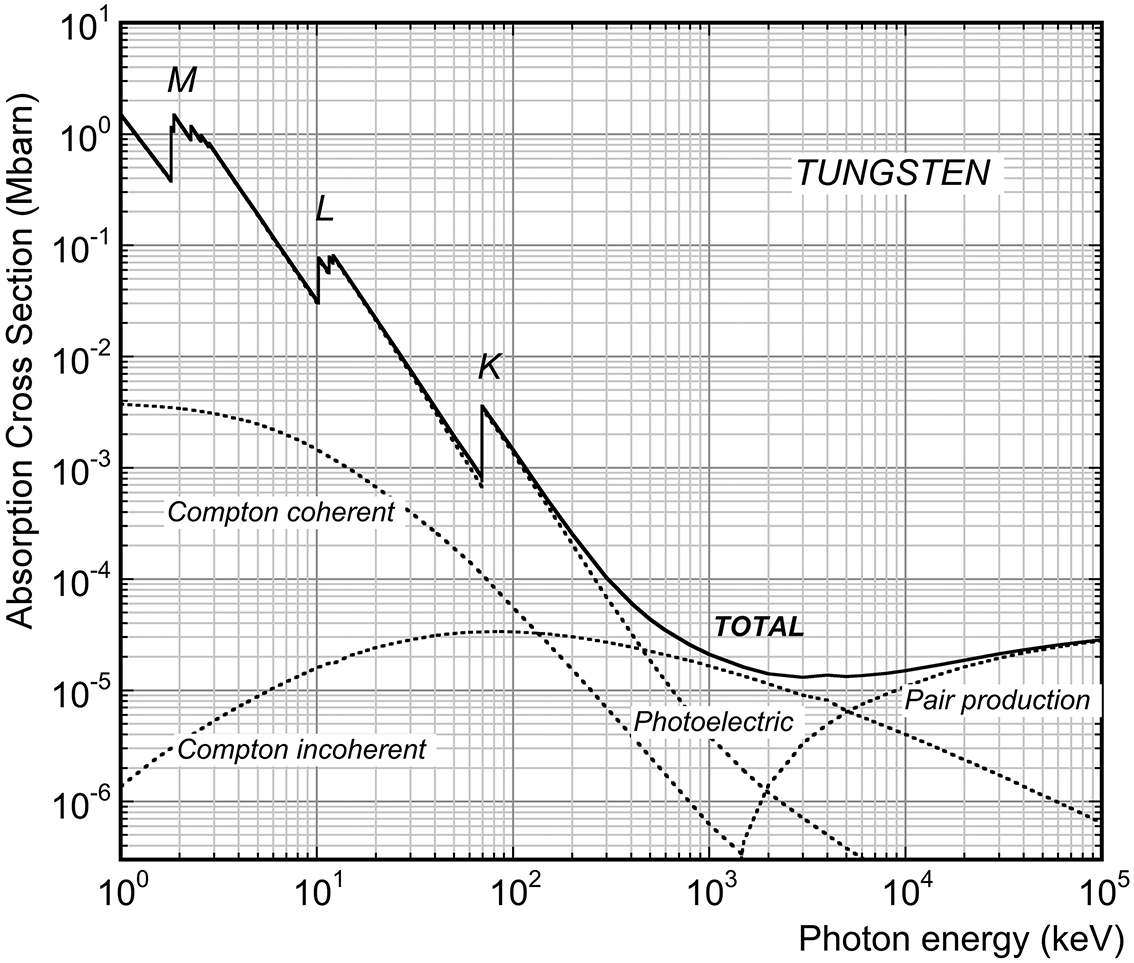
\includegraphics[width=\textwidth]{./plots/photon_cross_section.png}
		\caption{$\mathbf{\gamma}$\textbf{ interactions}}
		\label{fig:gamma-interactions}
	\end{subfigure}
	\hfill
	\begin{subfigure}[b]{0.575\textwidth}
		\centering
		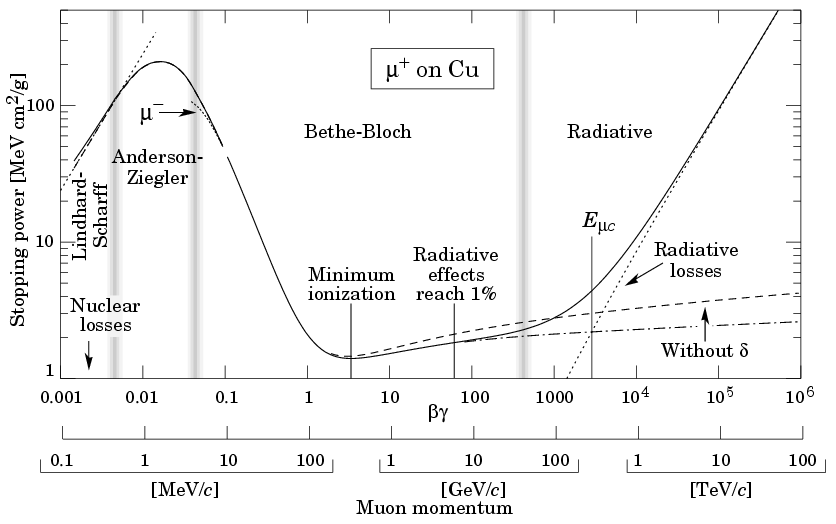
\includegraphics[width=\textwidth]{./plots/electron_ionisation_loss.png}
		\caption{$\mathbf{e^\pm}$\textbf{ interactions}}
		\label{fig:electron-interactions}
	\end{subfigure}
	\caption{\textbf{(a)} Cross section for different energy loss processes of a photon in tungsten. The sudden spikes correspond to the transition energy of 
	increasingly higher-energy electron shells. From \cite{chen2007interactions}. \textbf{(b)} Stopping power of copper, representatively on an antimuon $\upmu^+$, 
	with respect to its' momentum. Plot adopted with changes from \cite{meroli2017straggling}.}
	\label{fig:ionization-losses}
\end{figure}

\section{Hadronic showers}
\label{sec:heitler-matthews-model}

\section{Superposition principle}
\label{sec:superposition-principle}